% !TEX TS-program = pdflatex
% !TEX encoding = UTF-8 Unicode
\documentclass[11pt]{article} % use larger type; default would be 10pt

\usepackage[utf8]{inputenc} % set input encoding (not needed with XeLaTeX)
%
%%% PAGE DIMENSIONS
\usepackage{geometry} % to change the page dimensions

\geometry{a4paper} % or letterpaper (US) or a5paper or....,
%\geometry{margin=2in} % for example, change the margins to 2 inches all round
% \geometry{landscape} % set up the page for landscape
%   read geometry.pdf for detailed page layout information 
\usepackage{caption}
\usepackage{subcaption}
\usepackage{graphicx, xcolor} % support the \includegraphics command and options
\usepackage{siunitx}
%\usepackage[parfill]{parskip} % Activate to begin paragraphs with an empty line rather than an indent

%%% PACKAGES
\usepackage{booktabs} % for much better looking tables
%\usepackage{multirow}
\usepackage{array} % for better arrays (eg matrices) in maths
\usepackage{amssymb} % for math symbols (e.g. real numbers)
%\usepackage{paralist} % very flexible & customisable lists (eg. enumerate/itemize, etc.)
%\usepackage{verbatim} % adds environment for commenting out blocks of text & for better verbatim

\usepackage{wrapfig}

\usepackage{nameref}

\usepackage{color, soul}

\usepackage[backend=bibtex,sorting=none]{biblatex}
\bibliography{bibliography.bib}

%%% SECTION TITLE APPEARANCE
% (This matches ConTeXt defaults)
\usepackage{pdfpages}
\usepackage{hyperref}
\hypersetup{
  colorlinks=true,%activates colors
  allcolors=blue,%default color
  linkcolor=blue,
  filecolor=magenta,
  urlcolor=cyan,
}
%%% END Article customizations
%
%%% The "real" document content comes below...
%
\title{Memory effect in news' spreading networks: data analysis}
\author{Nicola Sella, Francesco Fanchin}
%\date{} % Activate to display a given date or no date (if empty),
         % otherwise the current date is printed
\begin{document}
\maketitle
\begin{abstract}
  Agent-based models (ABM) have been widely applied for complex systems
  modeling.
  A set of microscopic rules define agent's autonomous and
  cooperative actions: at a macroscopic level, the overall system
  exhibits the so-called ``emergent behaviour''.
  Rumour speading in networks is a natural environment where ABM
  could explain complex phenomena like echo chambers.
  Agents' memory is not generally taken into account by ABM
  literature: we do consider it in our analysis.
  As a starting point, we will rely on our previous work,
  ``Memory effects in news' spreading networks''.\\
  We developed a network framework where agents interact with themselves.
  Network's structure and the software codes were
  formerly explained: now we will pay particular attention to
  the connection between agents' memory length  and some of the
  network's statistical properties.
  Precisely we will measure, over different memory sizes, average
  clustering coefficient, diameter of the network and \hl{Gini index}
  of news' distribution .\\
  We will define a measurement procedure based on weighted
  regression; then we will suggest a phenomenological description for
  each of the measured quantities.
\end{abstract}
\thispagestyle{empty}
\newpage
\thispagestyle{empty}
\tableofcontents
\listoffigures
\listoftables
\newpage
\pagenumbering{arabic}
\section{Introduction}
Rumour spreading is a well-known phenomena in human interactions: its influence on public opinion and political elections is studied with different methodologies, derived from sociology, mathematics, physics, psicology and computer science.
DK model, (citazione), introduced by Dailey and Kendall, was one of the first attempts to mathematically reproduce the phenomena by stochastic differential equations: a famous variant is MK model.
With the development of complex networks, other approaches included network topology 
and different stochastic models like mean-field (cite) and interacting markov-chains (IMC)(cite).
Thanks to the rapid increasement in computing power, massive computer simulations have been made possible in most research and industry sectors.\\
Agent-based models (ABM) is a class of computational models for simulating the actions and interactions of autonomous agents.
Rumour spreading, in an ABM context, can be viewed as a network of interacting agents: from rules on single agent's behaviour,  a computer simulation will show the effects on the overall system.
This paper represents natural prosecution of the previous work,
''Memory effects in news' spreading networks'' by the same authors.\\
While the former described network's structure and agents' actions, this one clarifies the role of agents' memory length in network topology and news' distribution.
In the first section the focus will be on two network properties, average clustering coefficient and diameter.
In the second section we will point out the relation between memory size
and Gini index, to take into account inequalities within new's distribution. 
The whole model lacks, for the moment, of a validation with real data.

Does memory size have something connected with other properties?
we belive yes and we are expecting to find some correlations related
to information, spreading and entropy. Thus the use of Gini.\\ \\
Does a phenomenological approach make sense? \hl{Yes because abm needs
this type of approach (vedi slides)}\\ \\
Is this model validated with real data? \hl{Not yet.}
\hl{explain bubbles with image}
\newpage
\section{Effects on the network}
All agents in our network have a fixed \textit{memory length}, i.e.
they can remember a maximum amount of news;
in this section, memory length influence in network topology,
will be studied.\\
Clustering and diameter are standard measures in network science's
literarure and widely used to describe network properties.
Each of them will be plotted against memory length looking for
possible correlations.
All agents in our network have a fixed \textit{memory length}, i.e. they can remember a maximum
 amount of news.
In this section, its influence in network topology will be studied: clustering and
 diameter are standard measures in network science's literarure and widely used to describe 
 network properties.\\
  Each of them will be plotted 
 against memory length to search possible correlations.
\subsection{Clustering} \label{clustering}
A large number of networks show a tendency for link formation between neighboring vertices, 
i.e., the network topology deviates from uncorrelated random networks: this tendency is called 
\textit{clustering} \cite{clusterarticle}. \\
For unweighted graphs, the clustering of a node $u$ is the fraction of possible triangles over 
all possible triplets  through that node that exist \cite{clustersite},

\begin{equation}
\label{eq:clustering}
c_u = \frac{2 T(u)}{deg(u)(deg(u)-1)}
\end{equation}
where $T(u)$ is the number of triangles through node $u$ and $deg(u)$ is the degree of $u$.
Hence, the \textit{average clustering coefficient}  is:
\begin{equation}
\label{eq:average_clustering}
ACC = \frac{1}{n}\sum_{v \in G} c_v
\end{equation}
We ask wether memory, previously considered in section \ref{introduction}, could affect the 
average clustering coefficient.
To answer the question, the following experiment was designed:
for every memory size, five simulations were run over a thousand iterations; $ACC$'s mean and 
standard deviation were computed afterwards.\\
Finally, via weighted interpolation, a plot of $ACC$'s mean over memory size will show possible
 correlations. \hl{Results and discussion are reported together with diameter}.
\begin{figure}[h]
  \centering
  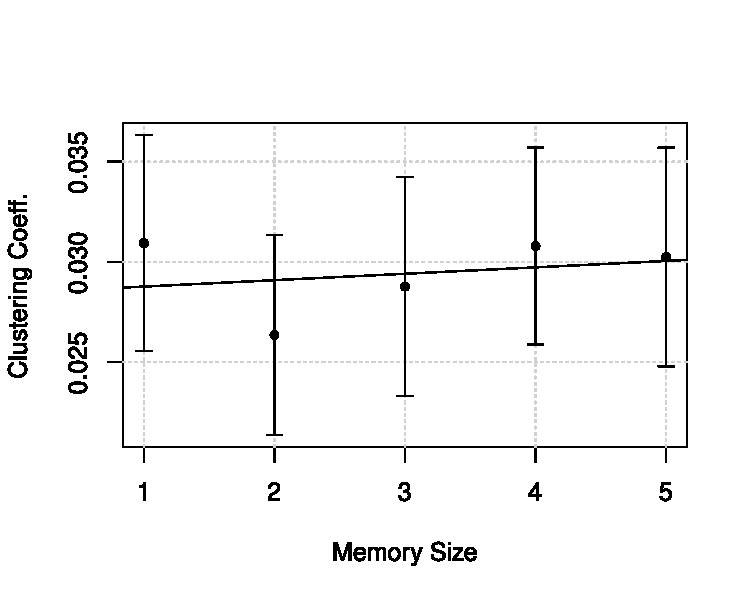
\includegraphics[trim={0cm 0cm 0cm 1cm},clip,width=.8\columnwidth]{img/clustering.pdf}
  \caption{$ACC$'s mean-memory size linear weighted fit: five simulations per point.}
  \label{fig:clustering}
\end{figure}

\section{Diameter}
kjhflh,jhv,jg

\newpage
\section{Effects on Users} \label{sec:users}
Every user can store a maximum amount of news, i.e. has a memory: this distinctive trait could affect news' distribution among users.
Indeed, if we insert in the network a certain number of news
(i.e. launching a simulation with some news), they will reach a
fraction of users (\textit{FOUR}, fraction of users reached)
at a fixed time.
\footnote{20 news for all of our simulations.}\\
News spreading over time, in general, starts with a fluctuating
transient and then reaches a stationary state: from a ``microscopic''
point of view, users' identity might vary but the fraction is
pretty much the same. \\
It is statistically correct to compute, for every news, the average
\textit{FOUR} over time, with a given threshold in order to
neglect the transient.\footnote{The end time and the threshold are
  experimentally determined by free trials. Moreover, threshold is
  not statistically significant since the end time was several orders of magnitude higher.}
Proceeding this way, we obtain a distribution of average \textit{FOURs}
for each news.\\
\section{Effects on news' distribution among users}
Memory selects the amount of news can be remembered: this could affect news' distribution among users.
Indeed, if we insert in the network a certain number of news (i.e. launching a simulation with many news), they will reach a fraction of users (FOUR, fraction of users reached) at a fixed time.\\
News spreading over time, in general, starts with a fluctuating transient and then reaches a stationary state: from a ``microscopic'' point of view, users' identity might vary but the fraction is pretty much the same. \\
It is statistically correct to compute, for every news, the average FOUR over time, with a certain threshold in order to neglect the transient ( the end time and the threshold are experimentally determined by free trials).
We obtain in this  way a distribution of average FOURs, one for each news.\\
Gini index measures the inequality of a distribution. Values of 0 and 1 stand for, respectively, the maximum homogeneity and the maximum heterogeneity.
However, this index is a function of random values: mean and error have to be estimated.\\
A certain number of samples is created by sampling with replacement of the average FOUR distribution: Gini index is computed for each one of them.
Now we have a population of Gini indexes, and we can extract mean and error: the whole process is known as bootstrap (see Appendix 1 for error estimation).\\
In practical terms, for every level of  memory, a simulation with twenty news is run out: Gini index' mean and error are computed like before.
The Gini index-memory plot shows a highly non-linear behaviour: sigmoid and gaussian seem to better represent data.\\
 In order to select the best-fit function, Chi-square is computed for both of them. \\
Because of asymmetric error bars, the optimization function is slightly different from the standard one, used for weighted interpolation: see Appendix 2 for more details.
Interpolation results are shown below:

%\begin{figure}[!h]
  %\centering
  %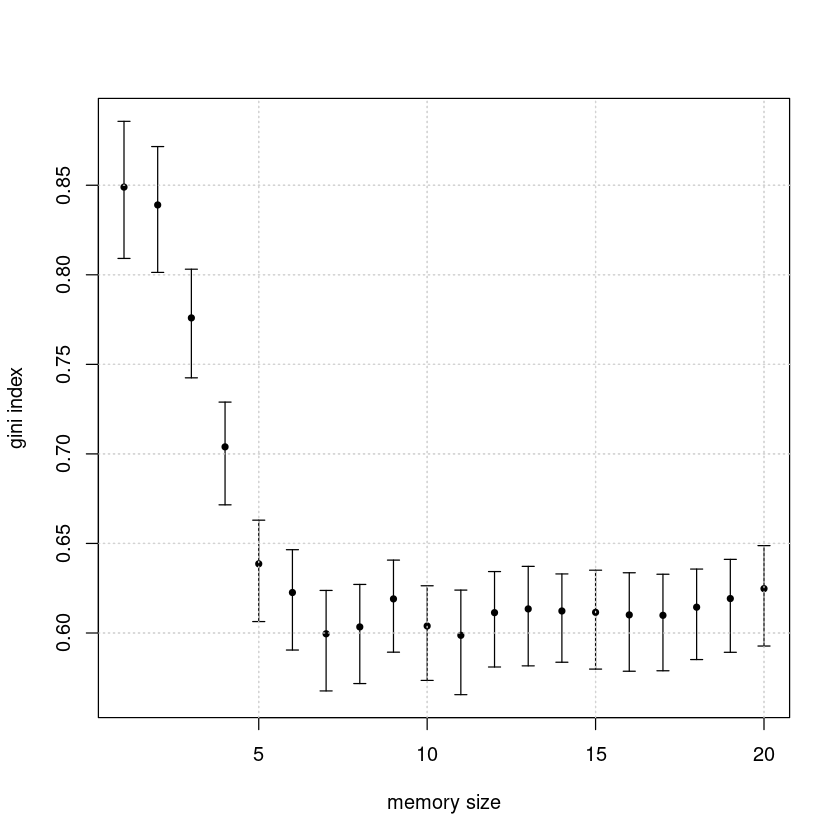
\includegraphics[width=.7\columnwidth]{img/gini_memory.png}
  %\caption{Gini index-memory plot with errorbars}
  %\label{fig:ginimem}
%\end{figure}

Risultati
subplot grafici??
manca grassetto/corsivo
immagini esplicative appendix2


\subsection{Appendix 1: errorbars for Gini index}

Bootstrap method is used to compute Gini index' mean and error: while for the former the process is pretty straigthforward, this is not the case for the latter.
Average FOUR distribution is asymmetrical and, in general, non-normal; we consider two different types of error.
Given N samples ${x_1,...,x_N}$ whose mean is $\mu$, correct standard deviation is:

$$
\sigma=\sqrt{\frac{\sum_{i=1}^{i=N}(x_i - \mu)^2}{N-1}}
$$


Quantile Standard Error (	QSE), instead, estimates the error by considering the fraction of samples falling within a certain interval: the whole distribution is divided in equal parts by a certain amount of ``quantiles''.\\
For example, in a Normal distribution, the interval $[\mu -\sigma, \mu +\sigma]$ ``covers'' approximately 68\% of the samples(figura...).
In ``quantiles'' terms (percentiles in this case), our errorbar starts from the $17^{th}$ percentile and ends in the $68^{th}$ percentile.\\
For non-normal distributions, standard deviation in general does not follow this property: to preserve it, we can compute QSE with the previous choice of quantiles, just by looking at the cumulative distribution, when values 0.17 and 0.68 are reached.

Immagini di gaussiana con 1 e 2 sigma e cumulativa della gaussiana...

The overall error is divided twofold, ``rightmost'' and ``leftmost''  the mean. For every part of the interval, we pick the ``largest'' between standard deviation and QSE: this conservative approach avoids underestimations in both directions.




\subsection{Appendix 2: asymmetric errorbars fitting}
The aim of a standard fitting problem is to find a function which reproduces experimental observations.
Let $f_{\theta}$ be the candidate function: $\theta=(\theta_1,...,\theta_m)$ is a vector of m parameters which completely determines function's values.
The optimization is performed with respect to $\theta$ parameters.\\
Given N datapoints with coordinates ${(x_i,y_i)}$ and y-errorbars $\sigma_i$, i=1,...,N, the usual optimization function for weighted interpolation is:

$$
E(\theta)= \sum_{i=1}^{N} \frac{(f_{\theta}(x_i)-y_i)^2}{\sigma_{i}^2}
$$


However, this formula is only applicable for gaussian errors, expressed by the standard deviation: in the problem we are facing, errorbars are not even symmetric.
We have developed an approximate optimization function which counts in this asymmetry.
In a weighted interpolation, the weight is the square inverse of the standard deviation: the ``shortest'' the errorbar, the closest will be $f(x_i)$ to $y_i$.
It might be an idea to split the error in two contributions, to be ``activated'' if the function value is greater or lower than the experimental value.
Let a and b be, respectively, the errorbars ``over'' and ``down'' the mean point: the optimization function for asymmetric errobars interpolation is:

$$
E= \sum_{i=1}^{N} \frac{(f(x_i)-y_i)^2}{a^{2}H(f(x_i)-y_i)+b^{2}H(y_i-f(x_i))}
$$

H(x) is the Heaviside function, which gives an ouput of 1 for $x>0$, 0 otherwise.\\
$f(x_i)$ ``sees'' an error of a if over $y_i$, or b if down.
The optimization is performed by specific R packages.

\subsection{Echo chambers}
In news media, \textit{echo chamber} is a metaphorical description
of a situation in which beliefs are amplified or reinforced by
communication and repetition inside a closed system.\cite{echochamwiki,echocham}\\
We qualitatively investigated the presence of echo chambers in our network.
First of all, our agents have a ``mental  state'', i.e. a vector of preferences: its components represent the amount of interest toward a certain topic.\\
 News have the same dimension of \textit{mental state vector} (MSVD) in order to establish a ``matching'' between news' topics and users' preferences.
 Mental state is highly involved in news' dynamics and network topology.\footnote{See section~\nameref{introduction} for more details on the previous work.}\\
 In the images below, for MSVD=3,5,7, we extracted main clusters from our network.
 Memory length is twelve for all the simulations.\\
 \textit{Modularity} is a measure for detecting community structure in graphs.\cite{modulwiki}
 To provide a comparison, nodes were painted with modularity class and the most recent news in memory.
 In case of news' homogeneity inside a single cluster, we are observing an echo chamber.\\
We can notice that number of clusters equals MSVD basically.
News' situation is more heterogenous: altough some clusters still exist, there is not a clear separation among users with different news.


\begin{figure}
  \centering
  \begin{subfigure}[t]{0.25\textwidth}
    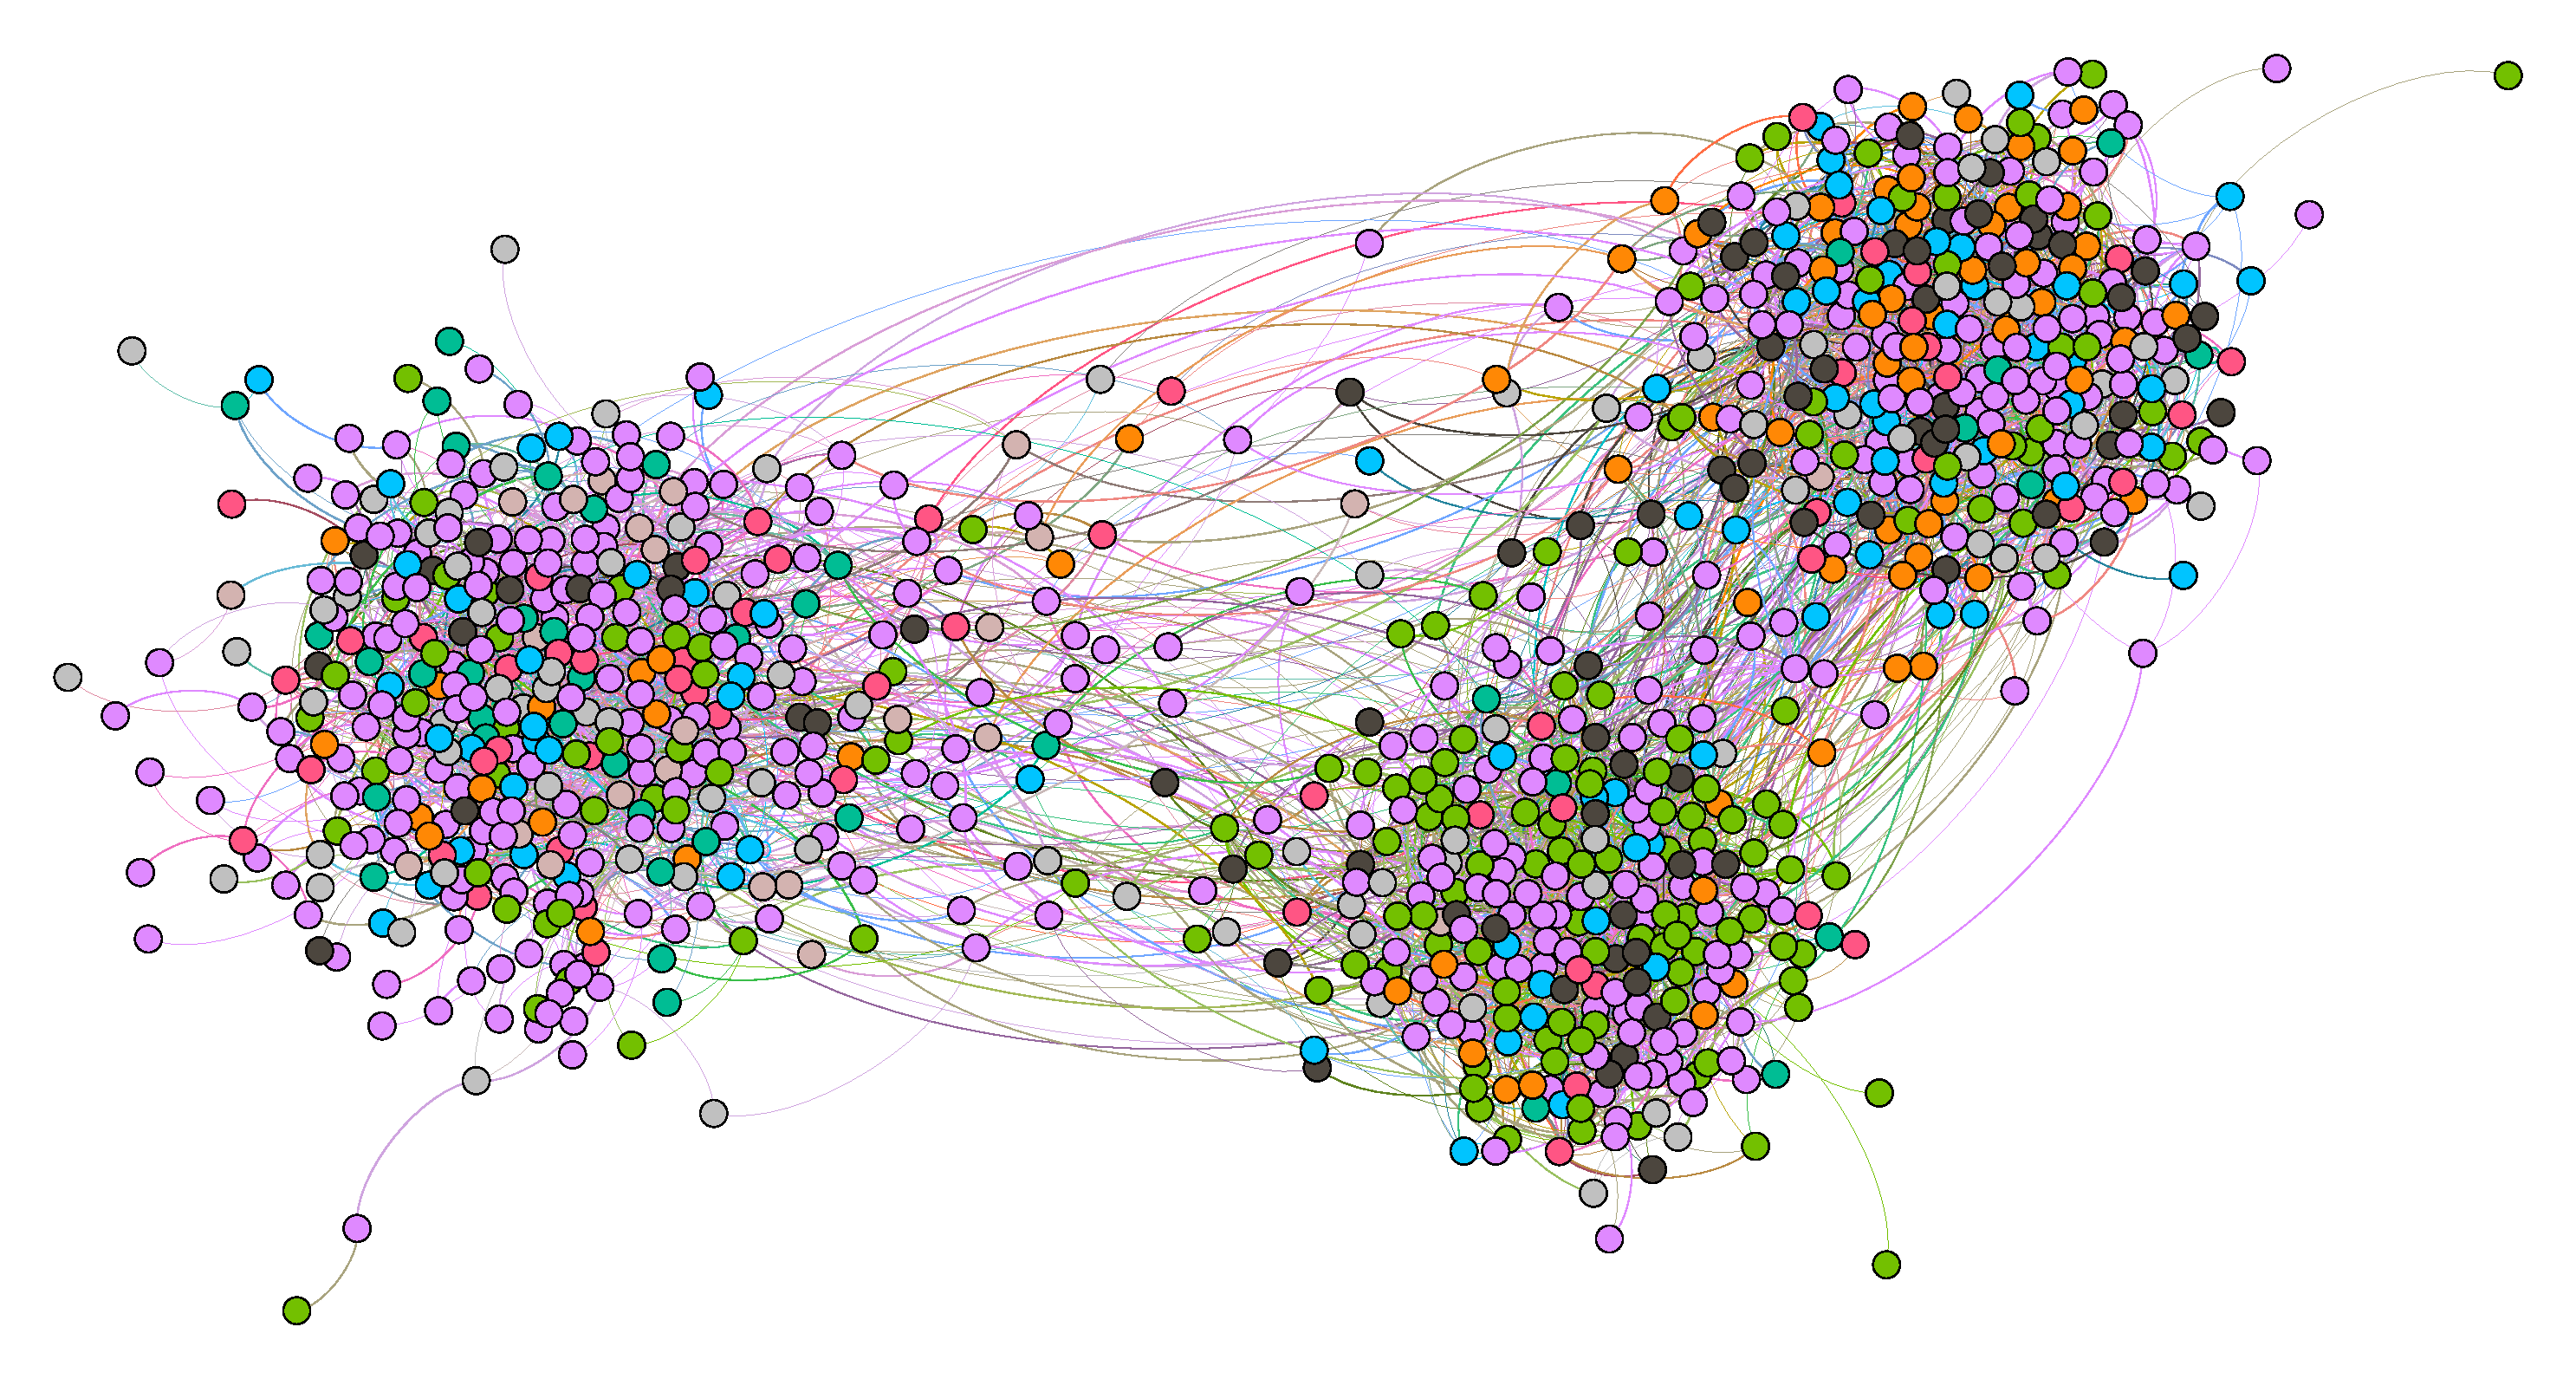
\includegraphics[width=\textwidth]{img/dim3_mod.pdf}
    \caption{bubble3mod}
    \label{fig:bubble3mod}
  \end{subfigure}
  ~
  \begin{subfigure}[t]{0.35\textwidth}
    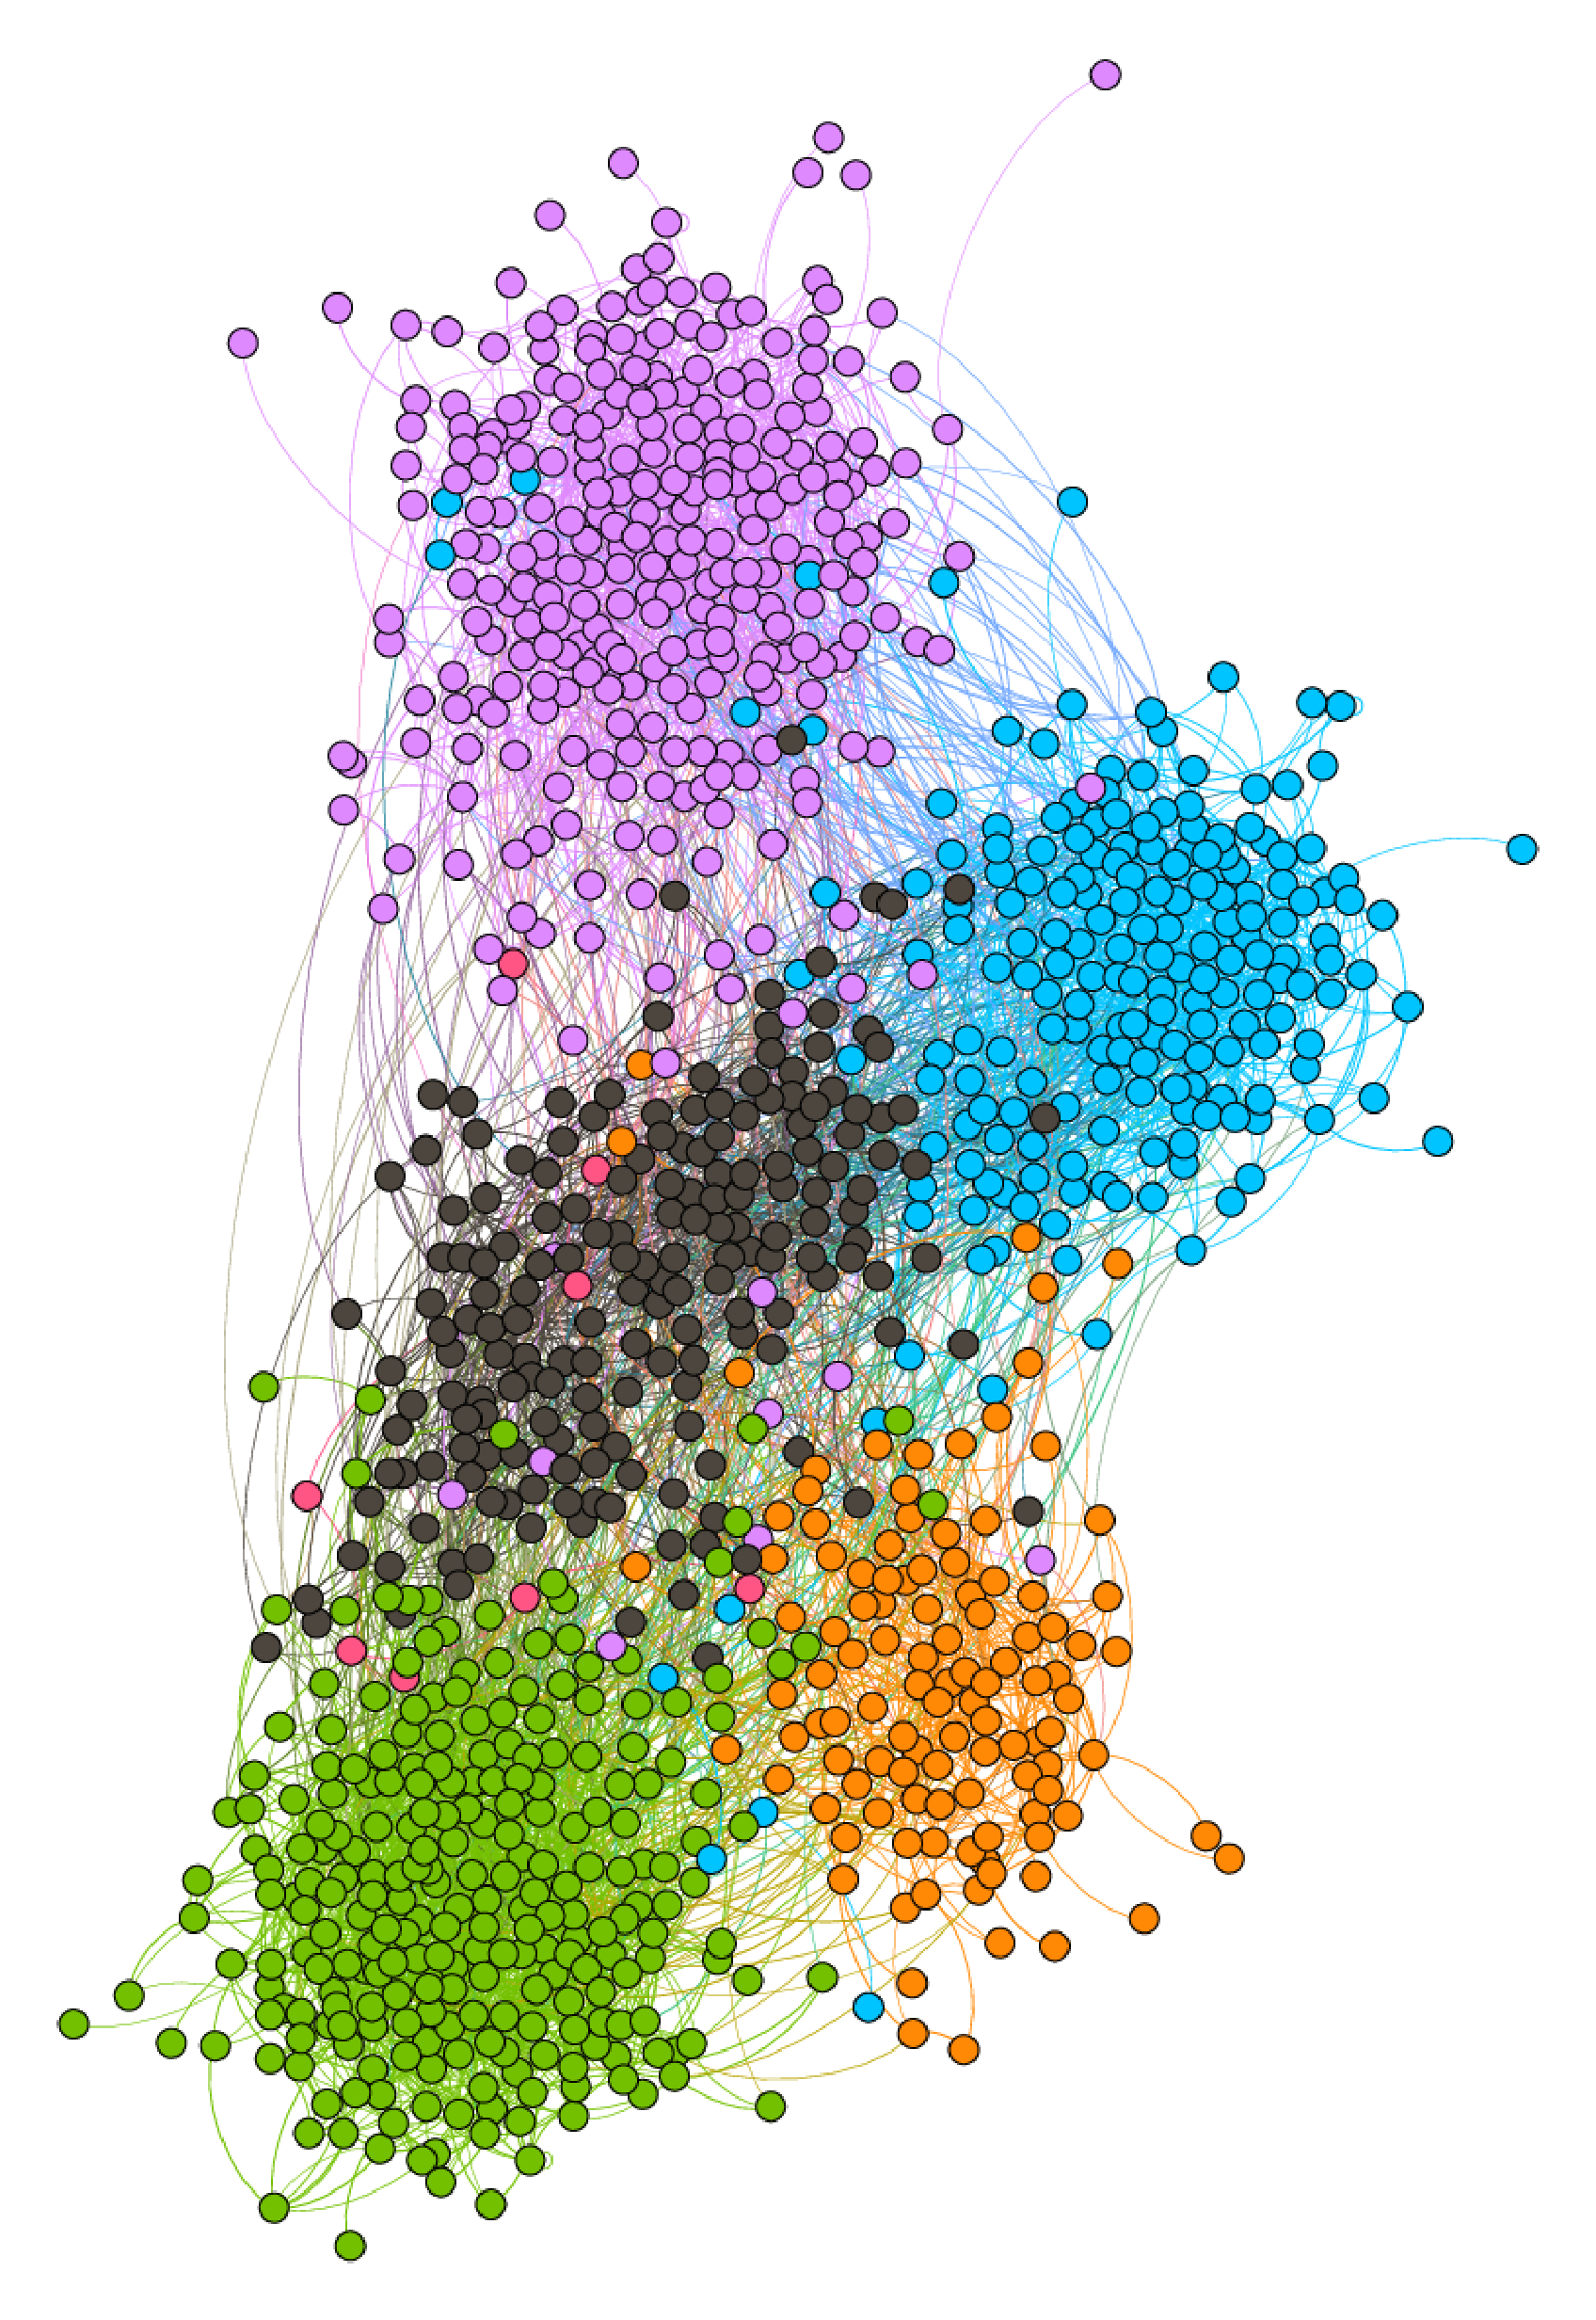
\includegraphics[width=\textwidth]{img/dim5_mod.pdf}
    \caption{bubble5mod}
    \label{fig:bubble5mod}
  \end{subfigure}
  ~
  \begin{subfigure}[t]{0.35\textwidth}
    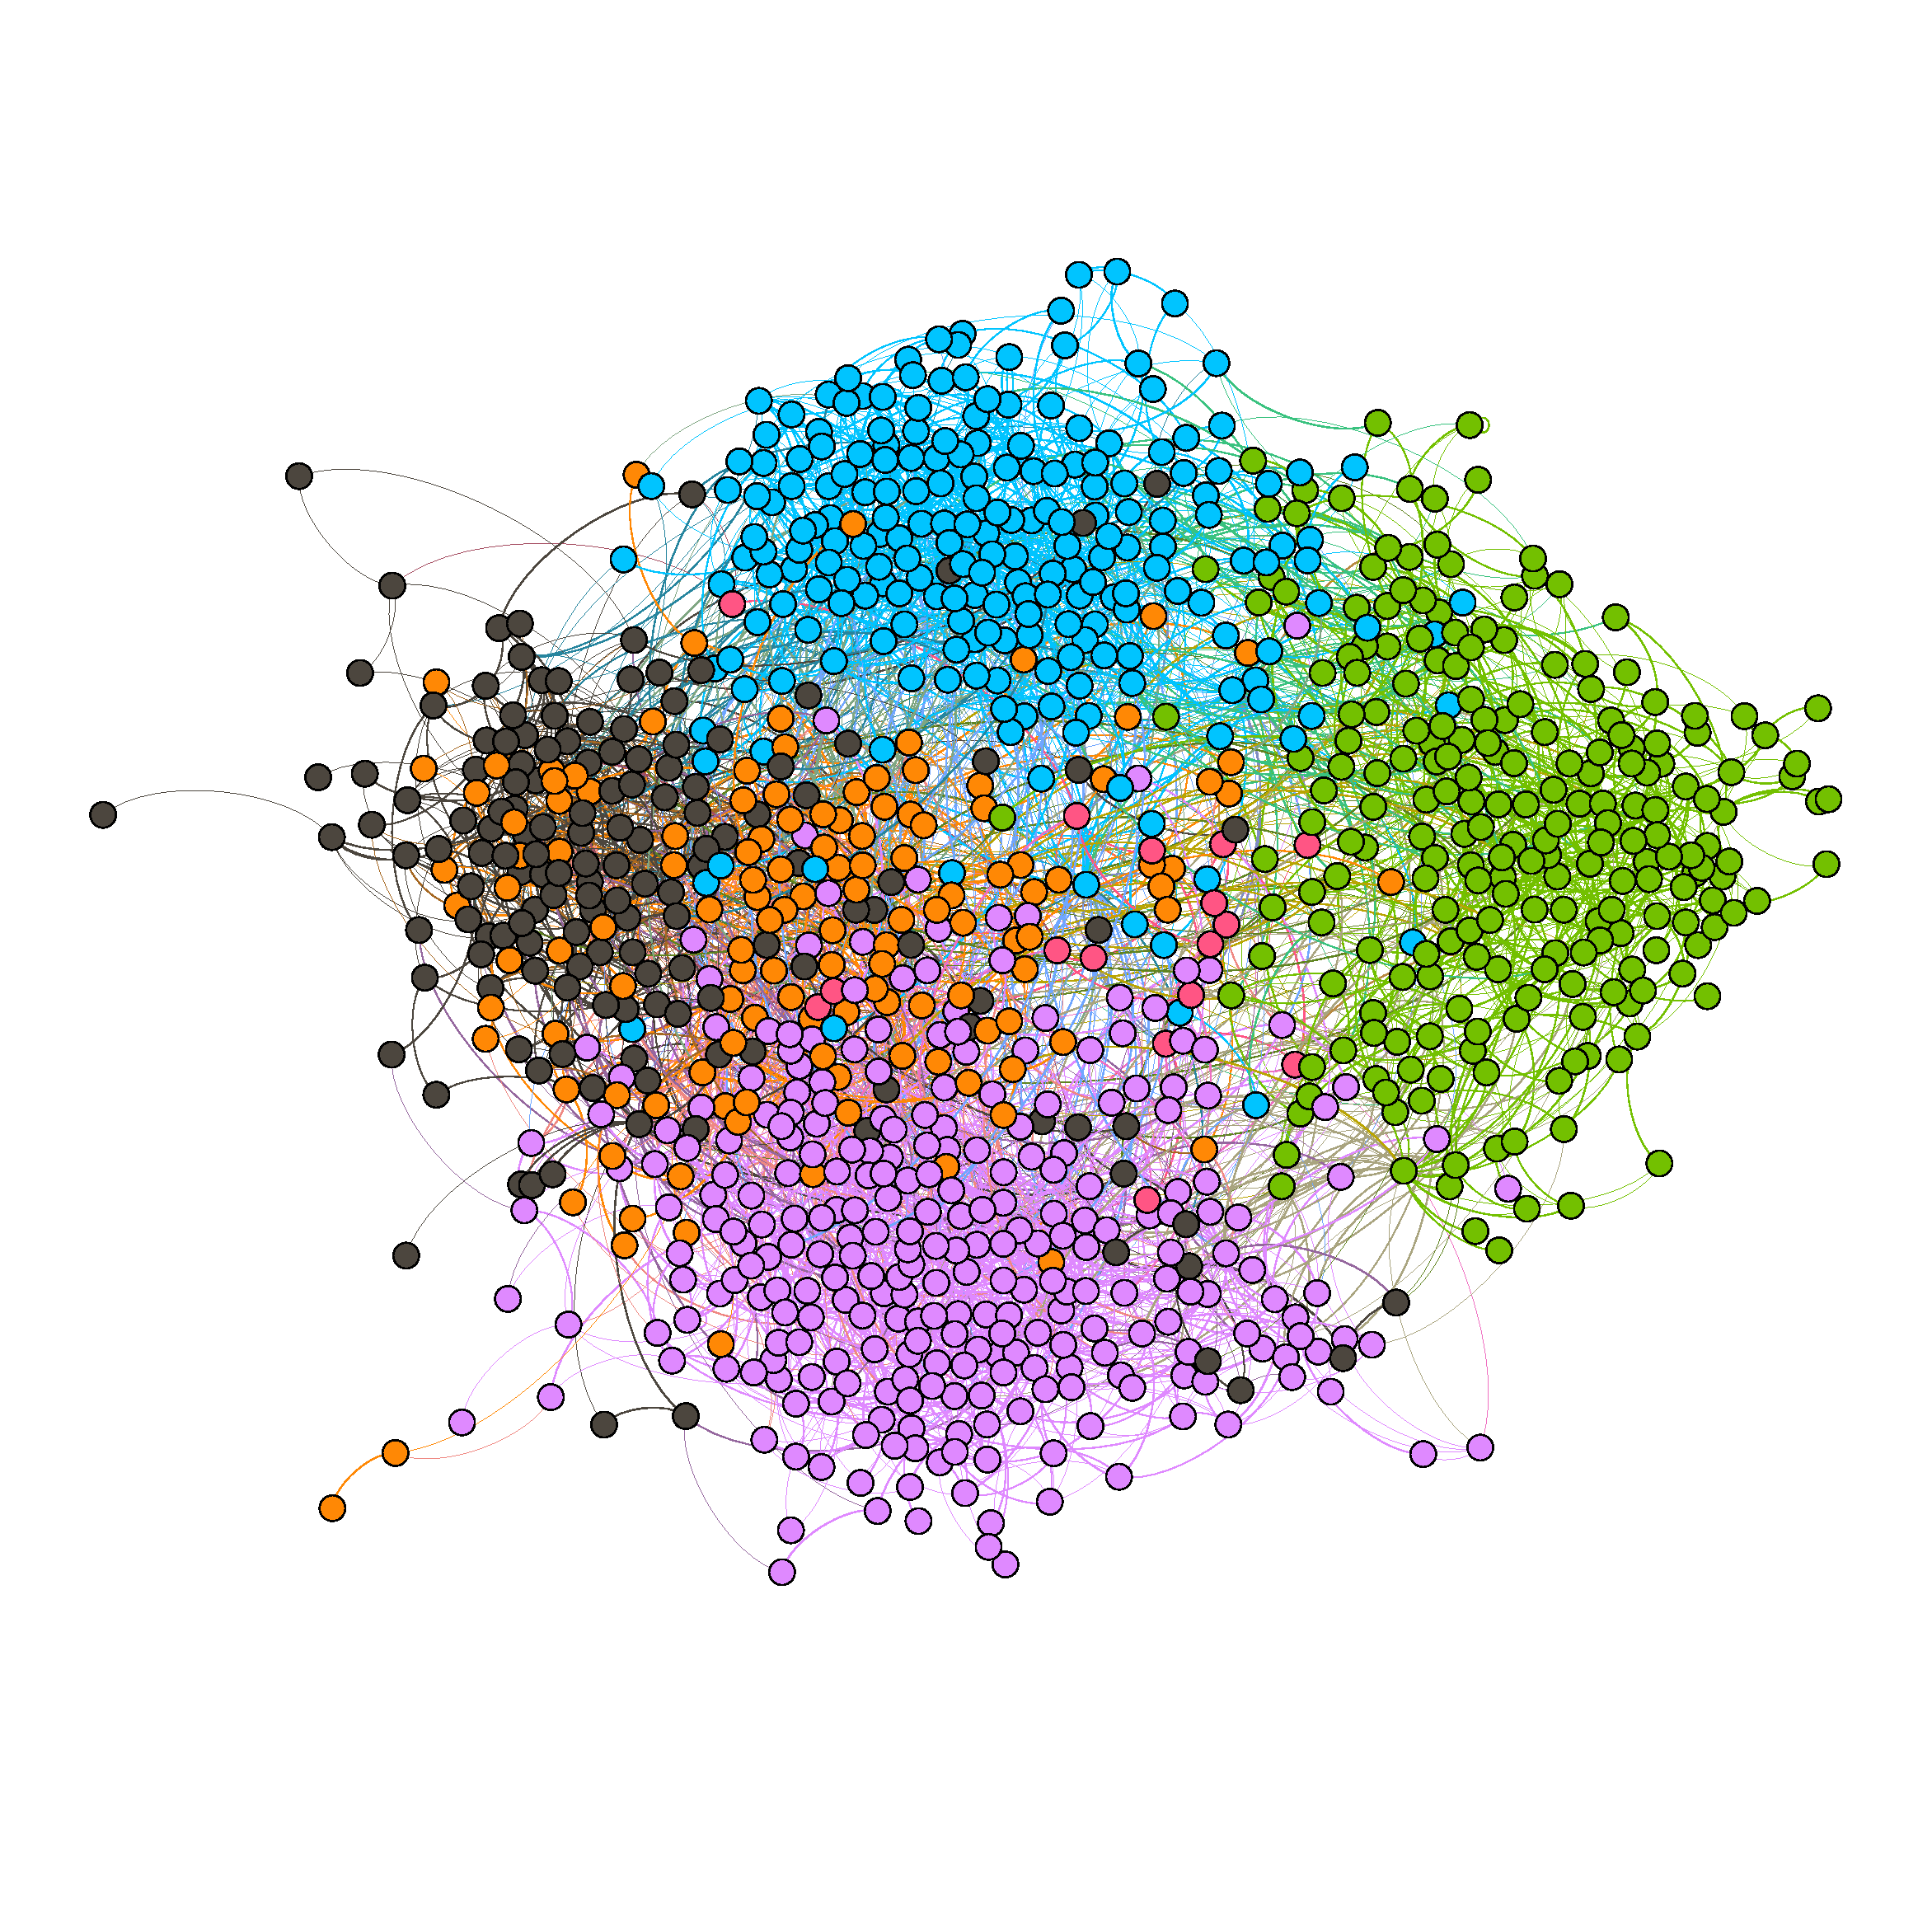
\includegraphics[width=\textwidth]{img/dim7_mod.pdf}
    \caption{bubble7mod}
    \label{fig:bubble7mod}
  \end{subfigure}
  \\
  \begin{subfigure}[t]{0.25\textwidth}
    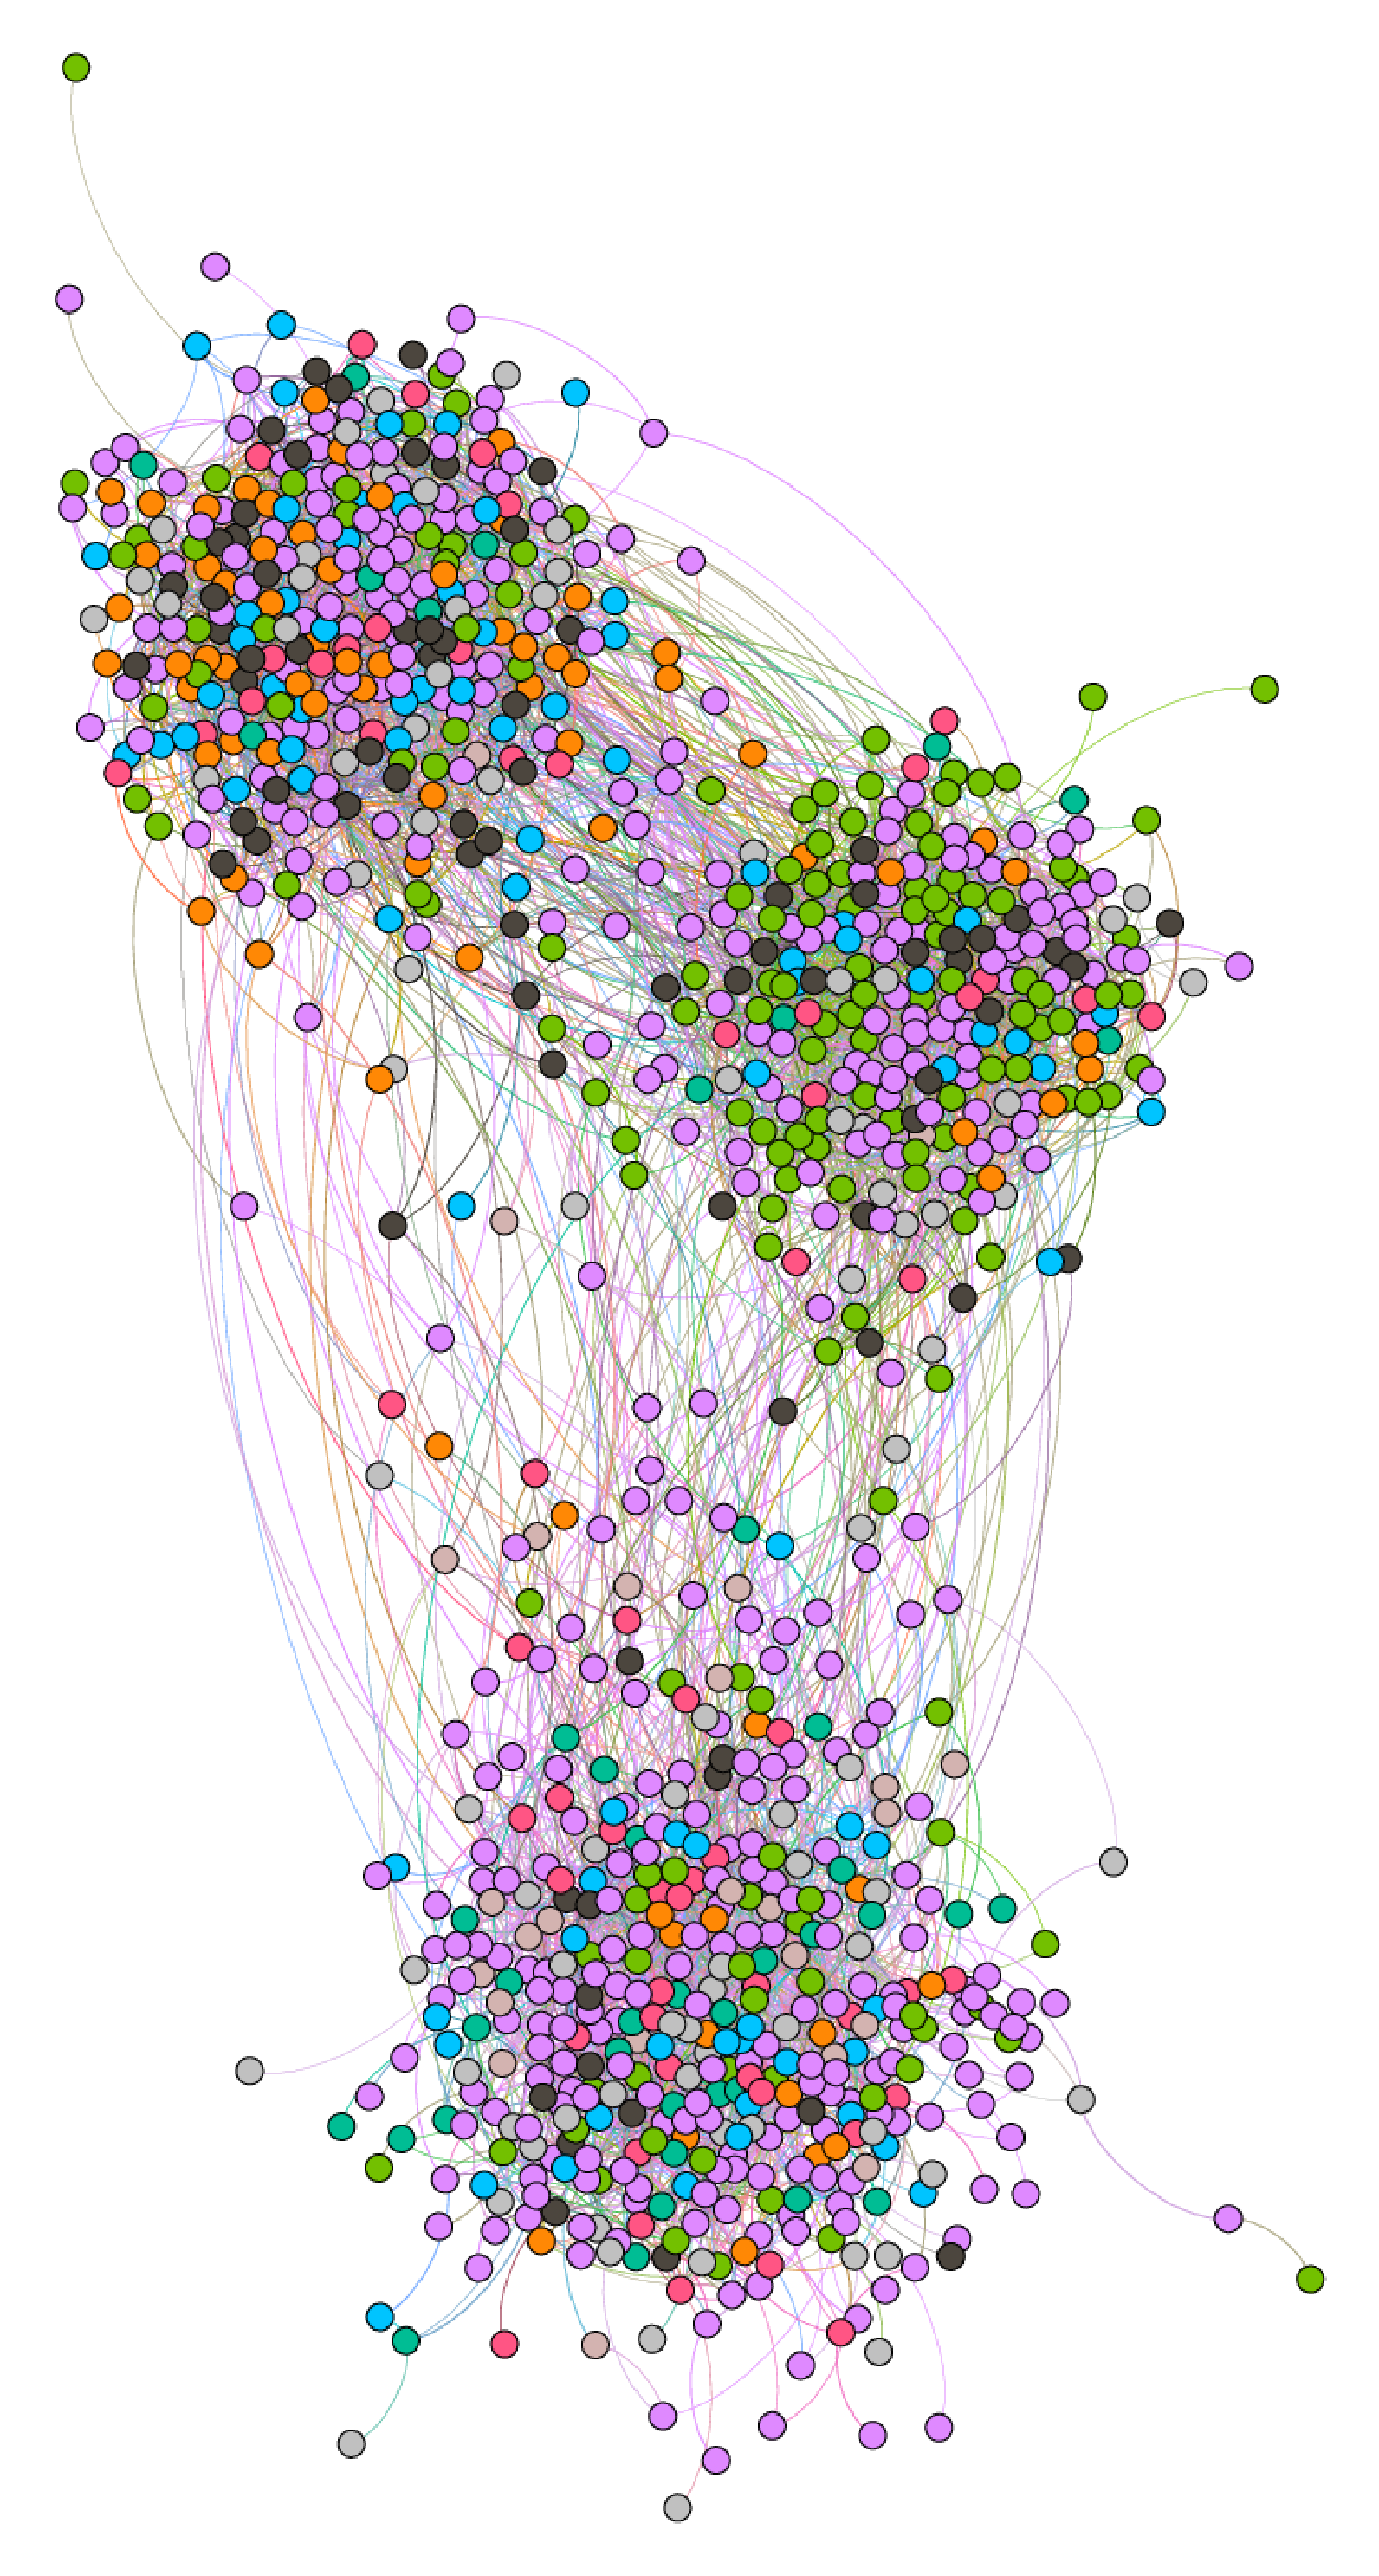
\includegraphics[width=\textwidth]{img/dim3_news.pdf}
    \caption{bubble3news}
    \label{fig:bubble3news}
  \end{subfigure}
  ~
  \begin{subfigure}[t]{0.35\textwidth}
    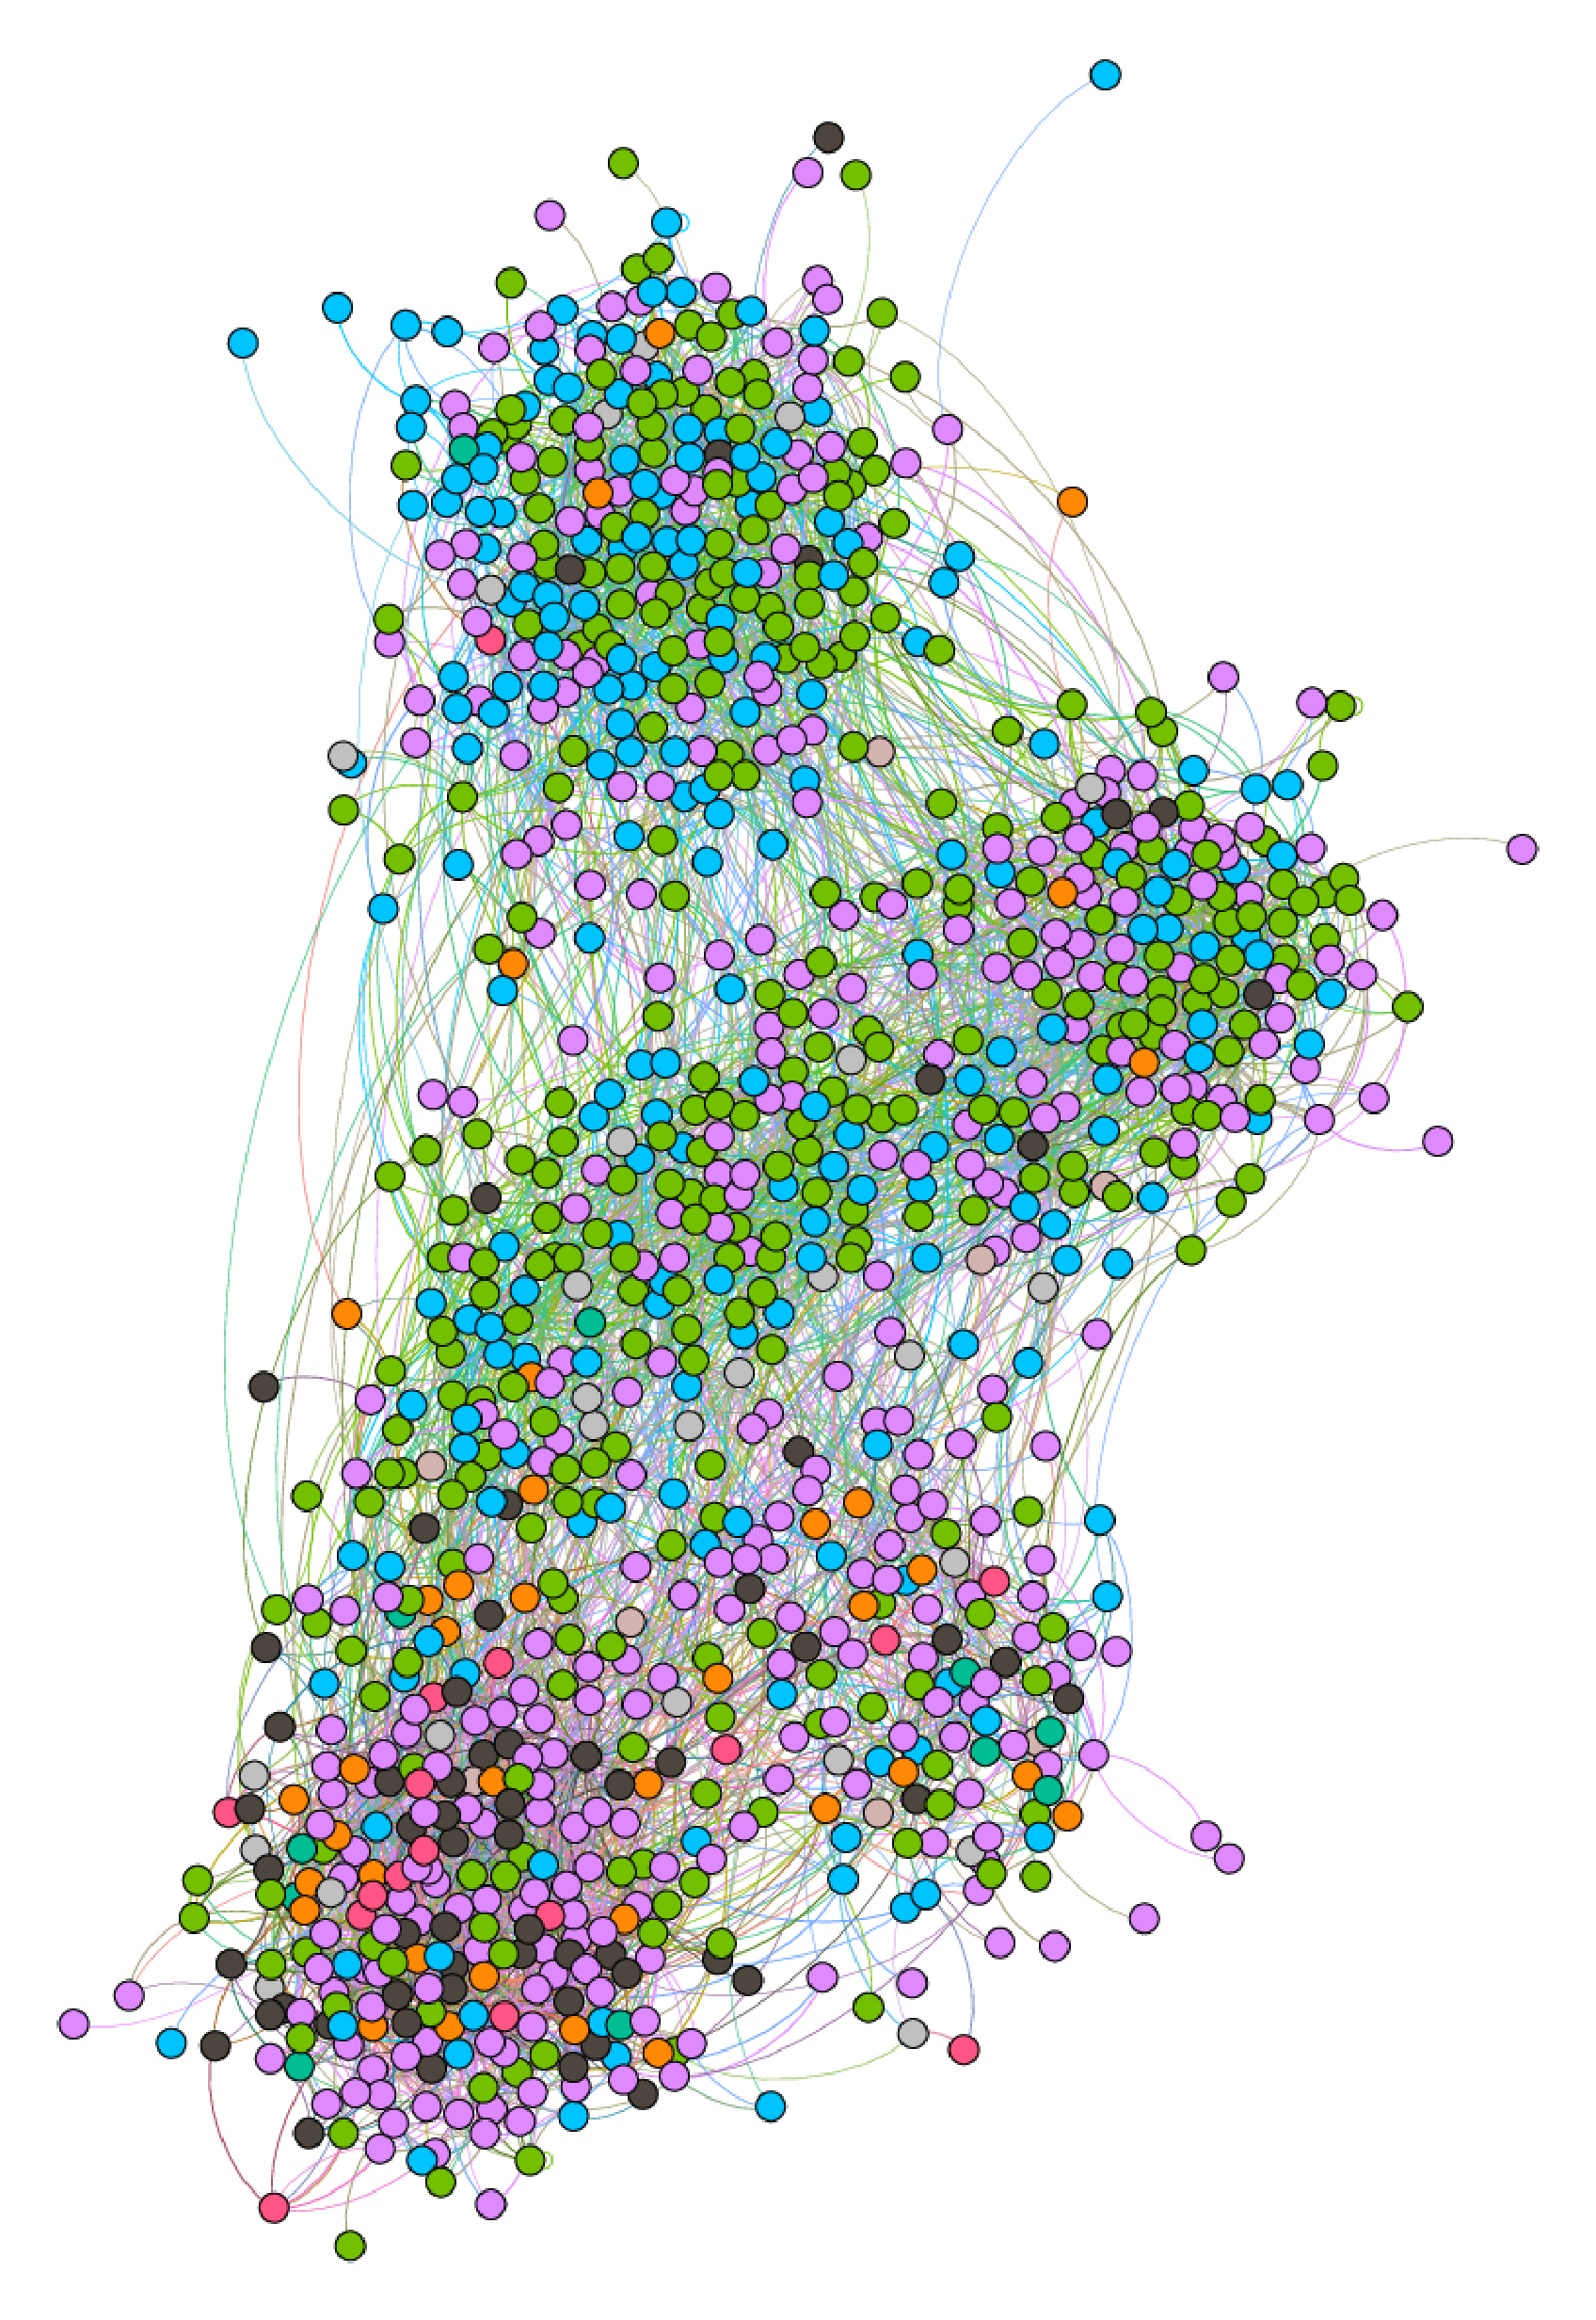
\includegraphics[width=\textwidth]{img/dim5_news.pdf}
    \caption{bubble5news}
    \label{fig:bubble5news}
  \end{subfigure}
  ~
  \begin{subfigure}[t]{0.35\textwidth}
    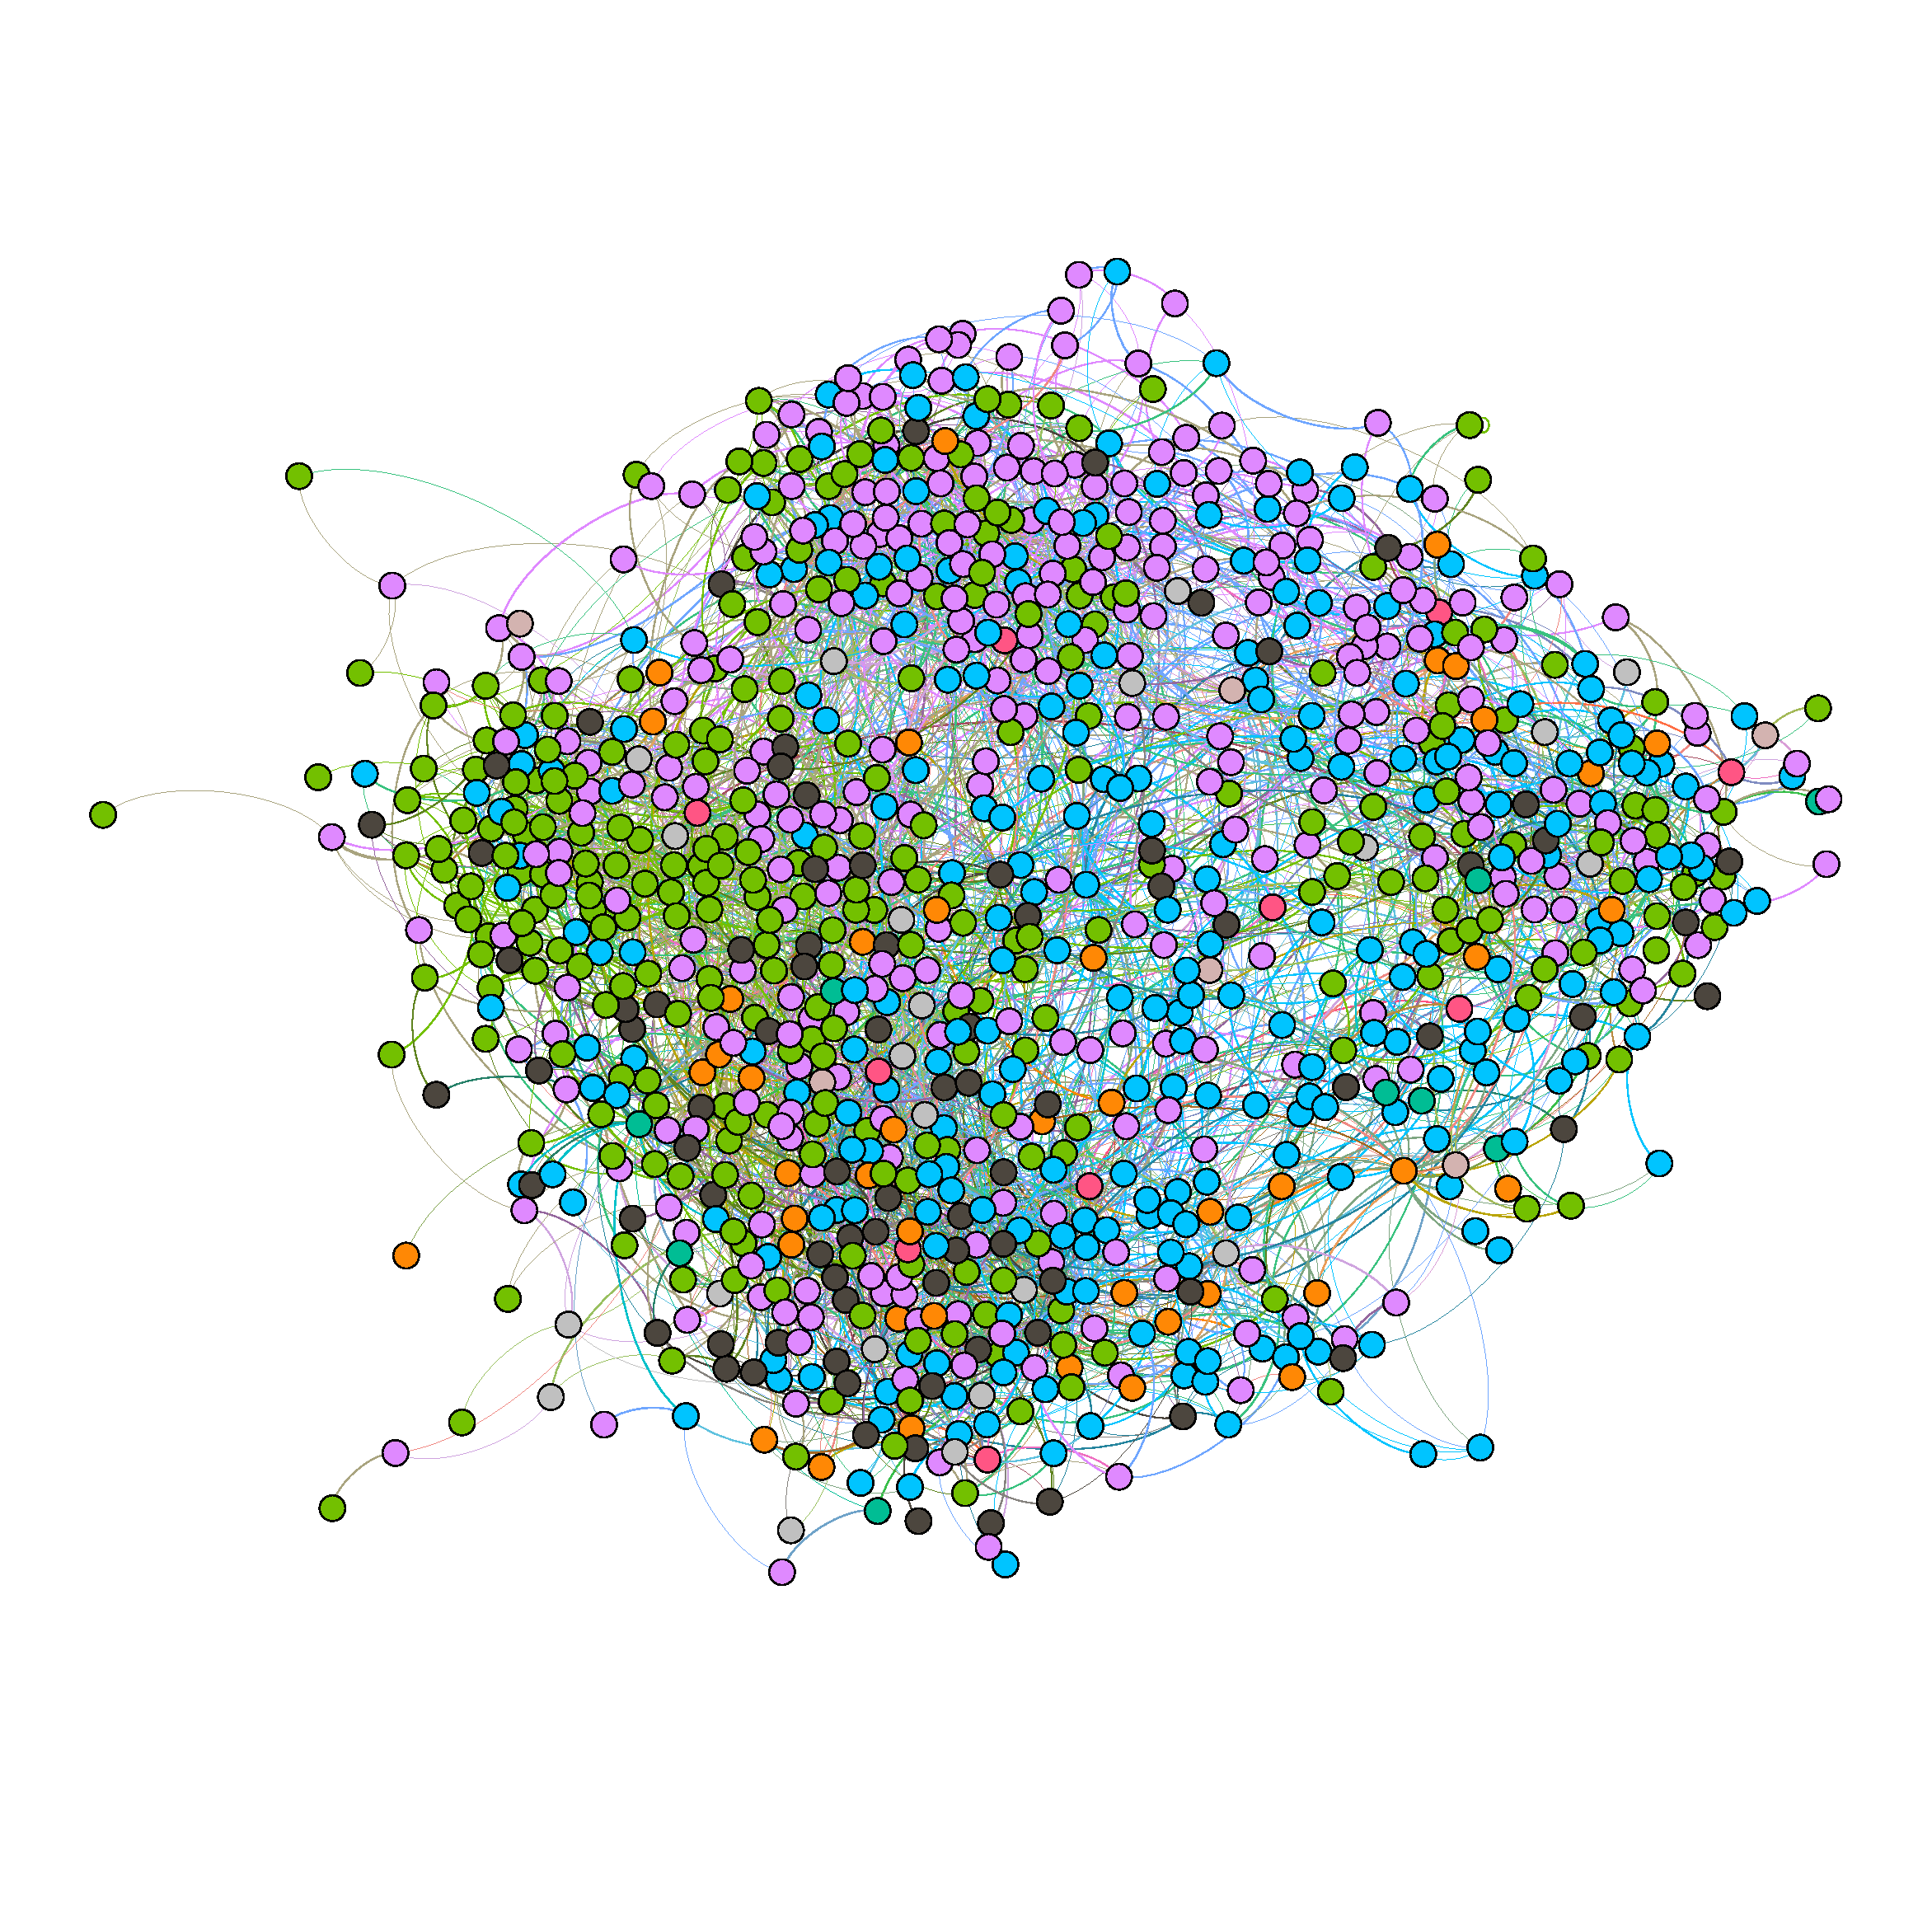
\includegraphics[width=\textwidth]{img/dim7_news.pdf}
    \caption{bubble7news}
    \label{fig:bubble7news}
  \end{subfigure}
  \caption[Network results: bubble chamber]{Simulations for 1000 users and 20 sources after 1000
    iterations. (\subref{fig:bubble3mod}), (\subref{fig:bubble5mod}) and
    (\subref{fig:bubble7mod}) highlights state vector.
    (\subref{fig:bubble3news}), (\subref{fig:bubble5news}) and
   (\subref{fig:bubble7news}) highlitghts different news.
  }
  \label{fig:test}
\end{figure}

\newpage
\section{Conclusion and further developments}
This paper has shown a correlation between memory length and Gini
index of news' distribution: a suitable optimization function
was developed in order to properly fit experimental data.
With reference to network topology, memory does not significantly
affect clustering and diameter.
There is not, at the moment, a clear evidence of echo chambers.\\
\\
Further developments include longer simulations with more nodes:
the overall system is not generally scale-invariant.
Hence, we expect different behaviors (like a more
distinct observation
of echo chambers) at higher orders of magnitude.\\
The presence of a phase transition in news' distribution could be investigated: in particular, the research should focus on its distinctive traits (critical exponents, order parameters...). 
In addition, other agents' actions or news' features could be added for a better realism.
For example, news are characterized by a certain amount of different topics.\\
However, they are not perceived as bad or good by agents: this additional ``degree of freedom''
could be inserted in the algorithm.

\newpage
\appendix
\section{Errorbars for Gini index}

\textit{Bootstrap} method\cite{bootstrap} is used to compute
\textit{Gini index}' mean and error: while for the former the process
is pretty straigthforward, this is not the case for the latter.
Average \textit{FOUR} distribution is asymmetrical and, in general,
non-normal; we consider two different types of error.
Given N samples ${x_1,...,x_N}$ whose mean is $\mu$,
\textit{correct standard deviation} is:
$\sigma=\sqrt{\frac{\sum_{i=1}^{i=N}(x_i - \mu)^2}{N-1}}$.\\
\textit{Quantile Standard Error} (QSE)\cite{quantile}, instead,
estimates the error by considering the fraction of samples
falling within a certain interval: the whole distribution is
divided in equal parts by a certain amount of ``quantiles''.\\
For example, in a Normal distribution, the interval
$[\mu -\sigma, \mu +\sigma]$ ``covers'' approximately $68\%$
of the samples \hl{(figura...)}.
In ``quantiles'' terms (percentiles in this case), our errorbar
starts from the $17^{th}$ percentile and ends in the $68^{th}$
percentile.\\
For non-normal distributions, standard deviation in general does
not follow this property: to preserve it, we can compute QSE with
the previous choice of quantiles, just by looking at the cumulative
distribution, when values 0.17 and 0.68 are reached.
\hl{Immagini di gaussiana con 1 e 2 sigma e cumulativa della gaussiana...}
\begin{table}[htpb]
  \centering
  \begin{tabular}{ccc}
    \toprule
    \textit{quantile} & $16\%$ & $84\%$ \\
    \midrule
    $10$   & 0.0130 & 0.00857 \\
    $10^3$ & 0.0239 & 0.00564 \\
    $10^5$ & 0.0236 & 0.00522 \\
    $10^7$ & 0.0236 & 0.00534 \\
    \bottomrule
  \end{tabular}
  \caption{quantile errors}
  \label{tab:quantile}
\end{table}
\begin{figure}[htpb]
  \centering
  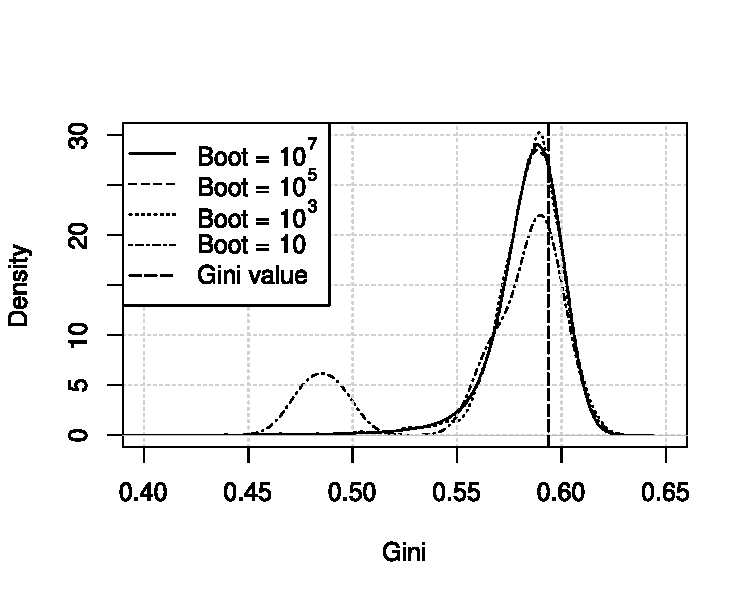
\includegraphics[width=.8\columnwidth]{img/bootstrap.pdf}
  \caption{Bootstrap}
  \label{fig:bootstrap}
\end{figure}
\begin{figure}[htpb]
  \centering
  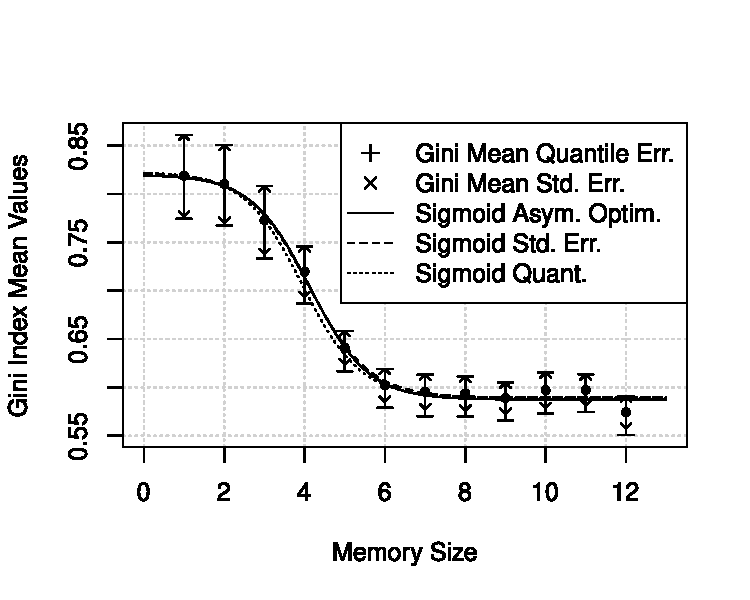
\includegraphics[width=.8\columnwidth]{img/appendix.pdf}
  \caption{errors gauss sigma}
  \label{fig:gauss_sigma}
\end{figure}
The overall error is divided twofold, ``rightmost'' and ``leftmost''
the mean. For every part of the interval, we pick the ``largest''
between standard deviation and QSE, see figure (\ref{fig:gauss_sigma}): this conservative approach avoids
underestimations in both directions.

\section{Asymmetric errorbars fitting}
The aim of a standard fitting problem is to find a function which
reproduces experimental observations.
Let $f_{\theta}$ be the candidate function:
$\theta=(\theta_1,...,\theta_m)$ is a vector of $m$ parameters which
completely determine function's values.
The optimization is performed with respect to $\theta$ parameters.\\
Given N datapoints with coordinates ${(x_i,y_i)}$ and y-errorbars
$\sigma_i$, $i$=1,...,N, the usual optimization function for
\textit{weighted interpolation}\cite{interpolation} is:
$$
E(\theta)= \sum_{i=1}^{N} \frac{(f_{\theta}(x_i)-y_i)^2}{\sigma_{i}^2}
$$
However, this formula is only applicable for gaussian errors,
expressed by the standard deviation: in the problem we are facing,
errorbars are not even symmetric.
We have developed an approximate optimization function which counts
in this asymmetry.
In a weighted interpolation, the weight is the square inverse of the
standard deviation: the ``shortest'' the errorbar, the closest will
be $f(x_i)$ to $y_i$.
It might be an idea to split the error in two contributions,
to be ``activated'' if the function value is greater or lower
than the experimental value.
Let a and b be, respectively, the errorbars \hl{``over'' and ``down''}
the mean point: the optimization function for \textit{asymmetric
  errobars interpolation} is:
$$ E= \sum_{i=1}^{N} \frac{(f(x_i)-y_i)^2}{a^{2}\mathcal{H}(f(x_i)-y_i)+b^{2}\mathcal{H}(y_i-f(x_i))} $$
$\mathcal{H}(x)$ is the \textit{Heaviside function},
$$\mathcal{H}(x):=\frac{\mathrm{d}}{\mathrm{d}x}\mathrm{max}
\{x,0\}:=\int_{-\infty}^x \delta (s) \mathrm{d}s$$ whose value
is zero for negative argument and one for positive argument.\\
The optimization is performed by an R implementation\cite{Roptim}
of textit{Nelder-Mead algorithm},\cite{neldermeadoriginal}
also known as textit{downhill simplex method} or
textit{amoeba}.\cite{neldermeadnumrec}\\
This algorithm is particularly appropriate for non-linear
optimization with many local minima.
\begin{figure}[htpb]
  \centering
  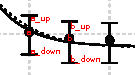
\includegraphics[width=.4\columnwidth]{img/err.pdf}
  \caption{error bars}
  \label{fig:errors}
\end{figure}

\newpage
\printbibliography
\end{document}